\documentclass[11pt]{article}
\usepackage{flushend}
\usepackage{amsmath,amssymb}
\usepackage{graphicx}
\usepackage{subcaption}
\usepackage{float}
\usepackage{mathtools}
\usepackage{empheq}
\newcommand*\widefbox[1]{\fbox{\hspace{2em}#1\hspace{2em}}}
\usepackage{hyperref}
\usepackage{fancyhdr}
\hypersetup{colorlinks=true,citecolor=magenta,linkcolor=red,urlcolor=blue}
\usepackage{geometry}
\geometry{a4paper,margin=1.0 in}
\usepackage[font={small,sf}]{caption}
\usepackage{IEEEtrantools}

%\providecommand{\keywords}[1]{\textbf{Keywords---} #1}
\setlength{\topmargin}{-0.05in}
\setlength{\textheight}{9.3in}
\raggedbottom
\newcommand{\rd}[1]{\mathop{\mathrm{d}#1}}
\DeclareMathOperator{\Res}{Res}

\begin{document}

\title{A study on Index Distribution in classical 1D Coulomb gas}
\author{UDDEEPTA DEKA\\
\small Summer Research Project report, June-August 2020\\
\small Mentor: Prof. Anupam Kundu\\
\small ICTS, Bengaluru	}
\date{} %% You could use \date{\small\today\today} to keep track
%% of preliminary versions
\maketitle
\pagestyle{myheadings}
\markboth{U.Deka}{A study on Index Distribution in classical 1D Coulomb gas}
\thispagestyle{empty}
\begin{abstract}
\noindent

In this study, we consider a 1-dimensional gas of \textit{N} particles confined by an external harmonic potential and interacting via the 1-D Coulomb potential (also known as 1-D one-component plasma model). Our aim is to find the probability distribution $\mathcal{P}(N_\mathcal{I})$ of the number of particles $N_\mathcal{I}$ confined in an interval $\mathcal{I} = [-a,a]$ on the real line. We calculate the saddle point density of particles analytically for large \textit{N} and compare it with our numerical results. This saddle point density is then used to find $\mathcal{P}(N_\mathcal{I})$.

\vspace{0.6 cm}
\end{abstract}

\tableofcontents

\section{Introduction}
A \textit{random matrix} is a $N\times N$ matrix with some or all its elements being random variables drawn from a probability distribution (in general this could be a joint distribution). This matrix upon diagonalisation, gives a set of eigenvalues $\{x_i\}$ which are random variables. One would then like to determine the joint distribution of these eigenvalues, $P(\{x_i\})$. Once $P(\{x_i\})$ is known, one could calculate several observables such as the spacing distribution of eigenvalues, distribution of largest eigenvalue, correlations between different eigenvalues, counting statistics etc. Thus, the central problem in random matrix theory (RMT) is to understand the spectral properties of the eigenvalues given the joint distribution of the entries.

In RMT, there are a number of distinguished ensembles for which the eigenvalue probability density function (PDF) can be calculated explicitly. One such ensemble is the Gaussian ensemble where the matrix elements are chosen independently from Gaussian distribution. Depending on the physical symmetries of the problem, three classes of matrices with Gaussian entries arise\cite{ref:mehta}: real symmetric (Gaussian Orthogonal Ensemble), complex Hermitian(Gaussian Unitary Ensemble) and self-dual Hermitian matrices (Gaussian Symplectic Ensemble). We are interested in Gaussian Unitary Ensemble (GUE). A random Hermitian $N\times N$ matrix $H$ is said to belong to the GUE if the diagonal elements and the upper triangular elements $h_{jk}=u_{jk}+iv_{jk}$ are independently chosen with PDFs:
$$
\frac{1}{\sqrt{\pi}}e^{-h_{jj}^2}\textrm{ and }\frac{2}{\pi}e^{-2(u_{jk}^2+v_{jk}^2)}=\frac{2}{\pi}e^{-2|h_{jk}|^2}
$$
respectively. The joint PDF of all the independent elements is
$$
\tilde{P}(H):=\prod_{j=1}^N\frac{1}{\sqrt{\pi}}e^{-h_{jj}^2}\prod_{1\leq j<k\leq N}\frac{2}{\pi}e^{-2|h_{jk}|^2} = A_N \prod_{j,k=1}^Ne^{-|h_{jk}|^2}= A_Ne^{-\textrm{Tr}(H^2)}
$$
where $A_N$ is the normalization. Clearly, $\tilde{P}(H)$ is invariant under a unitary transformation, that is, $\tilde{P}(U^{-1}HU)=\tilde{P}(H)$ for any unitary matrix $U$. For each realization of $H$, one has $N$ real eigenvalues $x_1,x_2,\dots,x_N$. The joint distribution of the eigenvalues can be calculated by making a change of variables from the entries to the eigenvalues and eigenvectors\cite{ref:mehta}. The eigenvectors decouple and the joint distribution of eigenvalues is of the form
\begin{equation}
P(x_1,\dots,x_N) = \frac{1}{Z_N}\exp\left(-\sum_{j=1}^Nx_j^2\right)\prod_{j<k}(x_j-x_k)^2
\end{equation} 
where $Z_N$ is the normalization factor. In general, the joint PDF for the eigenvalues from a Gaussian orthogonal (GOE), Gaussian symplectic (GSE) and Gaussian unitary ensemble (GUE) can be parameterized by the Dyson index $\beta$ and is given by
\begin{align}
P(x_1,\dots,x_N) &\propto \exp\left(-\frac{\beta}{2}\sum_{j=1}^Nx_j^2\right)\prod_{j<k}|x_j-x_k|^\beta\nonumber\\
\implies P(x_1,\dots,x_N) &\propto \exp\left[-\beta\left(\frac{1}{2}\sum_{j=1}^Nx_j^2-\sum_{j<k}\ln|x_j-x_k|\right)\right]\\
\implies P(x_1,\dots,x_N) &\propto \exp[-\beta E(\{x_i\})]
\end{align}
The Dyson index $\beta = 1,2,4$, respectively for GOE, GUE and GSE. However, we consider general matrix ensembles where $\beta >0$ can be arbitrary. This eigenvalue PDF can be identified with the Boltzmann factor of a particular log-gas known as one-component Coulomb system with the eigenvalues $\{x_i\}$ being interpreted as the particle positions. The energy of the system is given by
\begin{equation}
E(\{x_i\}) = \frac{1}{2}\sum_{j=1}^Nx_j^2-\frac{1}{2}\sum_{j\neq k}\ln|x_j-x_k|
\end{equation}
The first term can be interpreted as the potential energy due to a confining harmonic potential. We note that Coulomb potential in 2-D goes as $\sim\ln|x_j-x_k|$, so our system can be seen as consisting of charges with 2-D Coulomb interactions. Thus, the second term represents a pairwise logarithmic repulsion between charges. The first term scales as $O(N)$ for large N, whereas the second term scales as $O(N^2)$ since there are $N(N-1)$ pair of charges. For these two interactions to compete with each other we rescale $x_i$ as $x_i\to x_i\sqrt{N}$. This ensures that the $x_i$'s are of order $O(1)$. In these rescaled variables, the energy is given by
\begin{equation}
E(\{x_i\}) = \frac{1}{2}\left(N\sum_{j=1}^Nx_j^2-\sum_{j\neq k}\ln|x_j-x_k|\right)
\end{equation}
up to a constant. A detailed work on number statistics of the \textit{log-gas} system has been carried out by Dhar et.al.\cite{ref:dhar}. This model motivates us to change the form of the repulsive pairwise interaction and study certain observables. The classical 1-D one-component plasma (OCP) is an idealised system of $N$ identical charges on a line, with positions $\{x_i\}$, confined by an external harmonic potential and interacting pairwise via the 1-D repulsive Coulomb potential. That is, we replace the logarithmic pairwise repulsion $\ln|x_j-x_k|$ by the Coulomb repulsion in 1-D, which is a linear $|x_j-x_k|$ interaction. In our study, we look at the distribution of particles within a specified interval. The OCP has been extensively studied in literature because it can effectively model a variety of physical systems ranging from electrolytes and charge-stabilized colloids to dense stellar matter\cite{ref:oxford}. 


\section{1-D OCP model - joint distribution of eigenvalues}
We assume that the system is in thermal equilibrium such that the probability to observe the system in a configuration with particles at positions $\{x_i\}$ is given by the Boltzmann distribution
\begin{equation}
P(x_1,x_2,\hdots,x_N)=\frac{1}{Z_N}\exp[-\beta E(x_1,x_2,\hdots,x_N)]\label{eq-jpdf}
\end{equation}
where $\beta$ is the inverse temperature and $Z_N$ is the normalization constant. We consider ensembles of random matrices for which the energy of the configuration is given by
\begin{equation}
E(\{x_i\})=\frac{N}{2}\sum_{i=1}^Nx_i^2-\alpha \sum_{i\neq j}|x_i-x_j|\label{eq-energy}
\end{equation}
where $\alpha\geq 0$ denotes the strength of the Coulomb repulsion. For an ordered configuration $x_1<x_2<\hdots<x_N$, we can eliminate the absolute values to rewrite the energy function as
\begin{equation}
E(\{x_i\})=\frac{N}{2}\sum_{i=1}^Nx_i^2-2 \alpha \sum_{i>j} (x_i - x_j)
\end{equation}
The pairwise interaction term can be simplified as follows
\begin{align*}
\sum_{i>j} (x_i - x_j) &=\sum_{i>j}x_i - \sum_{i>j}x_j\\
& = \sum_{i=2}^N\sum_{j=1}^{i-1}x_i - \sum_{i=2}^N\sum_{j=1}^{i-1}x_j\\
\end{align*}
We look at the second term on the right
\begin{align*}
x_1 & \,\textrm{for i=2}\\
x_1 + x_2 &\,\textrm{for i=3}\\
x_1 + x_2 + x_3 & \,\textrm{for i=4}\\
\vdots\\
x_1 + x_2 + \hdots +x_{N-1}& \,\textrm{for i=N}
\end{align*}
Summing over all these terms we get
\begin{align*}
(N-1)x_1+(N-2)x_2+\hdots+{N-(N-1)}x_{N-1} & = \sum_{i=1}^N(N-i)x_i
\end{align*}
Thus, we get
\begin{align*}
\sum_{i>j} (x_i - x_j)& = \sum_{i=2}^Nx_i\left(\sum_{j=1}^{i-1}1\right)-\sum_{i=1}^N(N-i)x_i\\
& = \sum_{i=2}^Nx_i(i-1)-\sum_{i=1}^N(N-i)x_i\\
\therefore \sum_{i>j} (x_i - x_j) & = \sum_{i=1}^N(2i-N-1)x_i
\end{align*}
Finally, eq.\eqref{eq-energy} can be written as
\begin{equation}
E(\{x_i\})=\frac{N}{2}\sum_{i=1}^Nx_i^2-2 \alpha \sum_{i=1}^N(2i-N-1)x_i\label{eq-energy_modified}
\end{equation}
This form of the energy is used later in our numerical simulations for faster computing. Our quantity of interest is the number $N_\mathcal{I}$ of particles inside an interval $\mathcal{I}$. This is a random variable which can be expressed as 
$$N_\mathcal{I}=\sum_i\mathbb{I}_\mathcal{I}(x_i)$$
where $\mathbb{I}_\mathcal{I}(x_i)$ is the indicator function which equals 1 when $x_i\in \mathcal{I}$ and zero otherwise.


\section{Distribution of $N_\mathcal{I}$}
The probability density of $N_\mathcal{I}$ is given by
\begin{equation}
\mathcal{P}(N_\mathcal{I})=\int\prod_{i=1}^N\, dx_i\, P(\{x_i\})\delta\left[N_\mathcal{I}-\sum_{l=1}^N\mathbb{I}_\mathcal{I}(x_l)\right]\label{eq-prob_density}
\end{equation}
where $P(\{x_i\})$ is the joint PDF given in eq.\eqref{eq-jpdf}. We define the fraction of eigenvalues in the interval $\mathcal{I}$ as $\kappa_\mathcal{I}=N_\mathcal{I}/N$. The constraint that $N_\mathcal{I} = \kappa_\mathcal{I}N$ number of particles are in the interval $\mathcal{I}$ is forced using the $\delta$-function. Plugging eq.\eqref{eq-energy} into \eqref{eq-jpdf}, then plugging \eqref{eq-jpdf} into eq.\eqref{eq-prob_density}, we get
\begin{align*}
\mathcal{P}(N_\mathcal{I} = \kappa_\mathcal{I}N) &= \frac{1}{Z_N}\int\prod_{j=1}^Ndx_j\,\exp\left[-\beta\left(\frac{N}{2}\sum_{i=1}^Nx_i^2- \alpha \sum_{i\neq j}|x_i-x_j|\right)\right]\delta\left[N_\mathcal{I}-\sum_{l=1}^N\mathbb{I}_\mathcal{I}(x_l)\right]\\
&=\frac{Z_{N,\beta}(\kappa_\mathcal{I})}{Z_N}
\end{align*}
where
\begin{equation}
Z_{N,\beta}(\kappa_\mathcal{I}) = \int\prod_{j=1}^Ndx_j\,\exp\left[-\beta\left(\frac{N}{2}\sum_{i=1}^Nx_i^2- \alpha \sum_{i\neq j}|x_i-x_j|\right)\right]\delta\left[N_\mathcal{I}-\sum_{l=1}^N\mathbb{I}_\mathcal{I}(x_l)\right]\label{eq-znb}
\end{equation}
Expressing the $\delta$-function in Fourier representation,
$$
\delta(x-a) = \int_{-i\infty}^{i\infty}\frac{d\mu }{2\pi i}e^{\mu(x-a)}
$$ 
eq.\eqref{eq-znb} can be written as
\begin{align*}
Z_{N,\beta}(\kappa_\mathcal{I}) = \int\prod_{j=1}^Ndx_j\int_{-i\infty}^{i\infty}d\mu\, e^{-\beta E[\textbf{x},\mu,N_\mathcal{I}]}
\end{align*}
where the constants are being absorbed into the normalization factor. The energy function can now be written as
\begin{equation}
E[\textbf{x},\mu,N_\mathcal{I}] = \frac{N}{2}\sum_{i=1}^Nx_i^2- \alpha \sum_{i\neq j}|x_i-x_j|+\mu\left[\sum_{l=1}^N\mathbb{I}_\mathcal{I}(x_l)-\kappa_\mathcal{I}N\right]\label{eq-energy2}
\end{equation}
For coarse graining, we go to the continuum limit by defining the one-point and two-point densities, respectively, as follows
\begin{align}
\rho_N(x) &= \frac{1}{N}\sum_{i=1}^N\delta(x-x_i)\label{one-point-density}\\
\rho_{N,2}(x,x')&=\frac{1}{N(N-1)}\sum_{i\neq j}\delta(x-x_i)\delta(x'-x_j)\label{two-point-density}
\end{align} 
Using the properties of $\delta$-function and from eqs.\eqref{one-point-density},\eqref{two-point-density}, we can arrive at the following two identities for any arbitrary discrete function $f(x_i)$
\begin{align}
f(x_i) &= \int dx\,\delta(x-x_i)f(x)\nonumber\\
\implies \sum_i f(x_i) &= \sum_i\int dx\,\delta(x-x_i)f(x)\nonumber\\
\therefore \sum_i f(x_i) &=N\int dx\,\rho_N(x)f(x)\label{identity1}
\end{align}
\begin{align}
f(|x_i-x_j|) &= \int dx\,\int dx'\, \delta(x-x_i)\delta(x'-x_j)f(|x-x'|)\nonumber\\
\implies \sum_{i\neq j}f(|x_i-x_j|)&=\sum_{i\neq j}\int dx\,\int dx'\, \delta(x-x_i)\delta(x'-x_j)f(|x-x'|)\nonumber\\
\therefore \sum_{i\neq j}f(|x_i-x_j|)&=N(N-1)\int dx\,\int dx'\, \rho_{N,2}(x,x')f(|x-x'|)\label{identity2}
\end{align}
Using the identities \eqref{identity1} and \eqref{identity2}, we can express the energy in eq.\eqref{eq-energy2} in functional form as follows
\begin{align}
E[\textbf{x},\mu,N_\mathcal{I}] = & \frac{N^2}{2}\int_{-\infty}^\infty\rho_N(x)x^2\,dx-\alpha N(N-1)\int_{-\infty}^\infty \int_{-\infty}^\infty dx\, dx'\rho_{N,2}(x,x')|x-x'|\nonumber\\
& +\mu\left[N\int_a^b\rho_N(x)\,dx - \kappa_\mathcal{I}N\right]+\eta\left[N\int_{-\infty}^\infty\rho_N(x)\, dx-N\right]
\end{align}
where we have introduced a supplementary Lagrange multiplier $\eta$ to enforce the normalization condition on the density $\rho_N(x)$. $a$ and $b$, respectively, are the lower and upper bounds of the interval $\mathcal{I}$.

In the large-$N$ limit, the two-point density $\rho_{N,2}$ can be expressed in terms of one-point density $\rho_N$ as follows
\begin{align*}
\rho_{N,2}(x,x')&=\frac{N}{N-1}\rho_N(x)\rho_N(x')-\frac{1}{N-1}\rho_N(x)\delta(x-x')\\
&\sim \rho_N(x)\rho_N(x')
\end{align*} 
In this limit we can write $\rho_N(x) \approx \rho(x)$. We then rescale the Lagrange multipliers by $N$ and take $N^2$ common from all the terms to get
\begin{equation}
E[\textbf{x},\mu,N_\mathcal{I}]\sim N^2 S[\rho,\mu,\eta]
\end{equation}
where we have considered only the dominant $O(N^2)$ terms and neglected the subleading $O(N)$ terms. Here,
\begin{align}
S[\rho,\mu,\eta]=&\int_{-\infty}^\infty\rho (x)\frac{x^2}{2}\,dx-\alpha\int_{-\infty}^\infty\,dx\int_{-\infty}^\infty \, dx'\rho (x)\rho (x')|x-x'|\nonumber\\
&+\mu\left[\int_{a}^{b}\rho(x)\,dx-\kappa_I\right]+\eta\left[\int_{-\infty}^\infty\rho (x) \, dx-1\right]\label{eq-action}
\end{align}
is the \textit{action}. Effectively, we have now converted the multiple integral in eq.\eqref{eq-prob_density} into a functional integral over $\rho(x)$. The Jacobian of transformation from $x$ to $\rho(x)$ introduces terms of order $O(N)$ \cite{ref:forrester}, which are subdominant and we neglect them. Therefore, in the limit of large $N$, eq.\eqref{eq-prob_density} becomes
\begin{equation}
\mathcal{P}(N_\mathcal{I})=\frac{1}{Z_N}\int\mathcal{D}[\rho]\, d\mu\, d\eta\, e^{-\beta N^2 S[\rho,\mu,\eta]} 
\end{equation}
with the normalization factor 
\begin{align*}
Z_N = \int\mathcal{D}[\rho]\, d\mu \, d\eta e^{-\beta N^2S[\rho,\mu=0,\eta]}
\end{align*}
We note that in calculating the normalization constant, there is no additional constraint imposed by $\mu$. In the large-$N$ limit the functional integral over $\rho$ may be evaluated by the saddle-point method. To do this, we need to find the density that minimizes the action.


\section{Numerical simulation of the saddle-point density profile}
The configuration energy for $N$ particles is given by eq.\eqref{eq-energy_modified}. However we also have the Lagrange multiplier $\mu$, which can be thought of being analogous to a chemical potential. The energy of the configuration then becomes
\begin{equation}
E(\{x_i\})=\frac{N}{2}\sum_{i=1}^Nx_i^2-2 \alpha \sum_{i=1}^N(2i-N-1)x_i+\mu\sum_{i=1}^N \mathbb{I}_\mathcal{I}(x_i)\label{eq-energy_simulation}
\end{equation}
We consider the interval to be symmetric about 0 i.e., $\mathcal{I}=[-a,a]$. The third term on R.H.S. implies that we add $\mu$ for every particle lying inside the interval $\mathcal{I}$ for a given configuration.

In order to find the saddle-point density profile at thermal equilibrium, we make use of the Markov Chain Monte Carlo (MCMC) method. A Markov Chain is a chain of random transitions in which the next state is only dependent on the current state, i.e., the system has no memory. A Monte Carlo method is the one that involves a stochastic sampling. The most common implementation of MCMC is via the \textit{Metropolis-Hastings algorithm}. With this algorithm one chooses a random point in parameter space to jump to. If the likelihood at the new point is higher than that of the current point, then one makes a jump. If the likelihood at the new point is lower, then one can also make a jump, but with a probability given by the ratio of the likelihoods at the new and old points. The likelihood in our problem is given by $\exp[-\beta E(\{\textbf{x}_i\})]$. 

The Metropolis-Hastings algorithm for the simulation is implemented as follows:
\begin{enumerate}
	\item \emph{Initialization}: We start with $N$ particles generated from a normal distribution centered around 0 with unit standard deviation. This consitutes our initial configuration $\textbf{x}_i$.
	\item \emph{Fixing values of parameters}: We fix $a,\beta,\alpha$ and $\mu$.
	\item \emph{Modifying the configuration}: We randomly select one particle from the sample and change its location by a random amount, $\Delta x_i$, generated from a uniform distribution between $[-1/\sqrt{N},1/\sqrt{N}]$, and call this new configuration $\textbf{x}_n$.
	\item \emph{Calculating the energy change}: We calculate the energy of both configurations $\textbf{x}_i$ and $\textbf{x}_n$ using eq.\eqref{eq-energy_simulation} and call them $E_i$ and $E_n$ respectively. The difference is given by $\Delta E=E_n-E_i$.
	\item \emph{Accept/reject}: We generate a random number, $r$, from a uniform distribution between 0 and 1. If $r<\exp\left(-\beta\Delta E\right)$, we accept the new configuration and make a transition. This is our new $\textbf{x}_i$. This completes one realization. 
	\item \emph{Repeat}: We start with this accepted configuration as our initial configuration for the next realization. We repeat steps 3 through 5 for reasonable number of realizations. We calculate the acceptance ratio:
	$$
		\frac{\textrm{Cumulative number of realizations for which the new configuration is accepted}}{\textrm{Total number of realizations}}
	$$
	at each realization.
	\item \emph{Collecting data}: For convergence, we expect the acceptance ratio to become constant after a finite number of realizations. We collect data points after every $2N$ realizations. We discard those data points for which the acceptance ratio has not become constant.
\end{enumerate}
Simulations are carried out for $N=\{100,200,500\}$ particles for various values of $\mu=\{0,\pm 1,\pm 50,\pm 200\}$. We consider $2\times 10^5$ realizations for $100$ particles, $4\times 10^5$ realizations for $200$ particles and $10^6$ realizations for $500$ particles. The parameters are set at: $\alpha=1,\beta=1,a=1$. The convergence check is illustrated in Appendix \ref{MCMC convergence} for a few combinations of $N$ and $\mu$.
\begin{figure}[H]
	\centering
	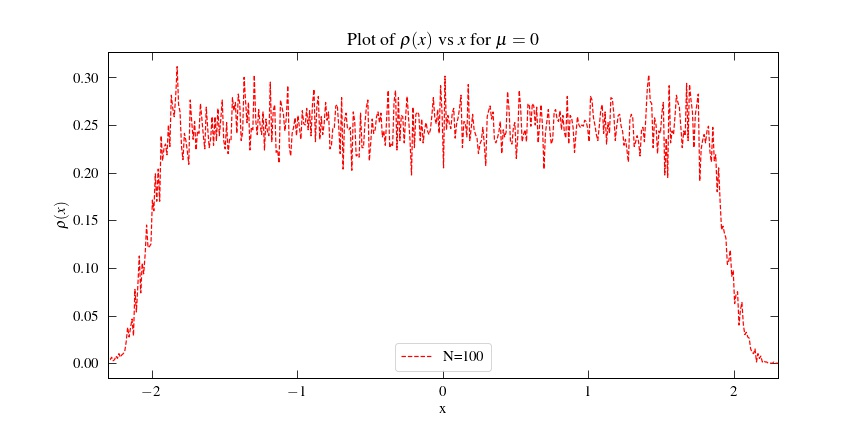
\includegraphics[width=0.8\columnwidth]{m00.jpg}
	\caption{Saddle point density profile for $\mu=0$}
	\label{fig:mu0}
\end{figure}
\begin{figure}[H]
	\centering
	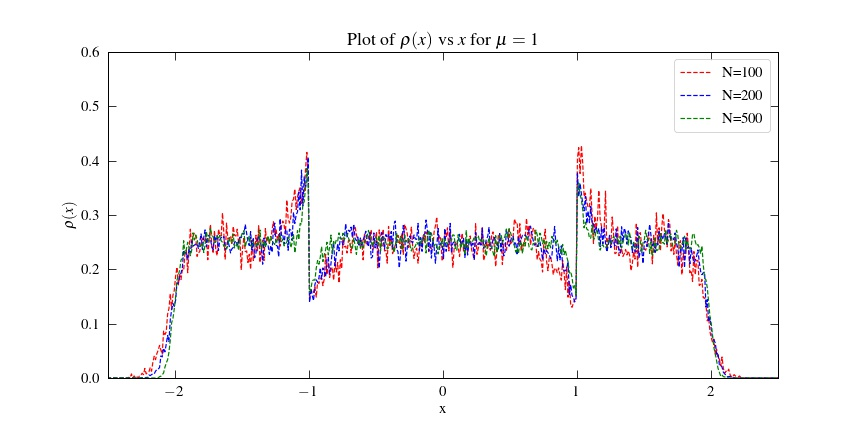
\includegraphics[width=0.8\columnwidth]{m1.jpg}
	\caption{Saddle point density profile for $\mu=1$}
	\label{fig:mu1}
\end{figure}
\begin{figure}[H]
	\centering
	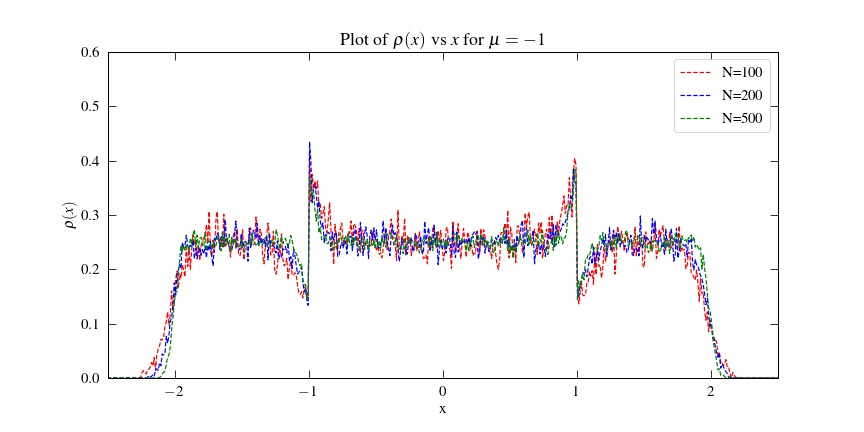
\includegraphics[width=0.8\columnwidth]{m-1.jpg}
	\caption{Saddle point density profile for $\mu=-1$}
	\label{fig:mu-1}
\end{figure}
\begin{figure}[H]
	\centering
	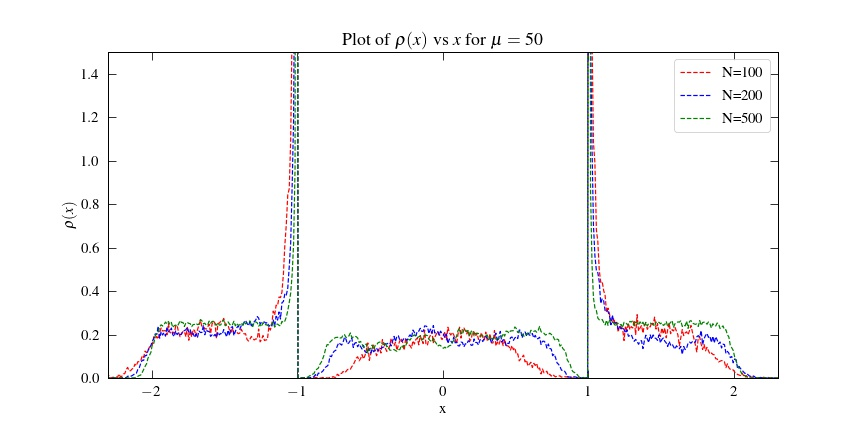
\includegraphics[width=0.8\columnwidth]{m50.jpg}
	\caption{Saddle point density profile for $\mu=50$}
	\label{fig:mu50}
\end{figure}
\begin{figure}[H]
	\centering
	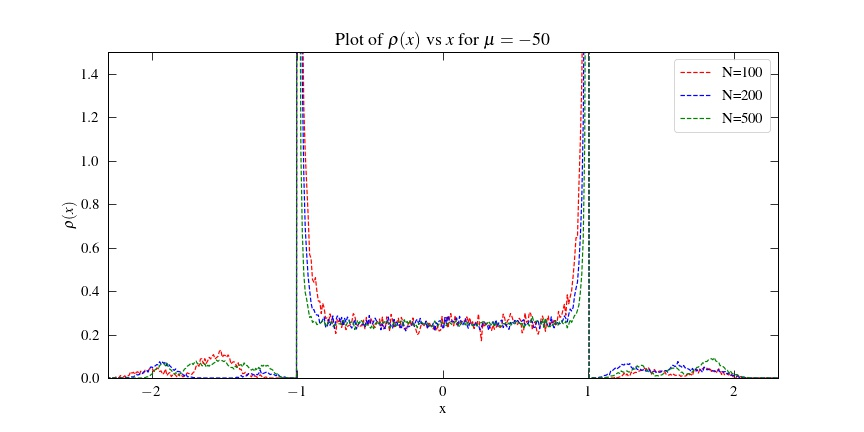
\includegraphics[width=0.8\columnwidth]{m-50.jpg}
	\caption{Saddle point density profile for $\mu=-50$}
	\label{fig:mu-50}
\end{figure}
\begin{figure}[H]
	\centering
	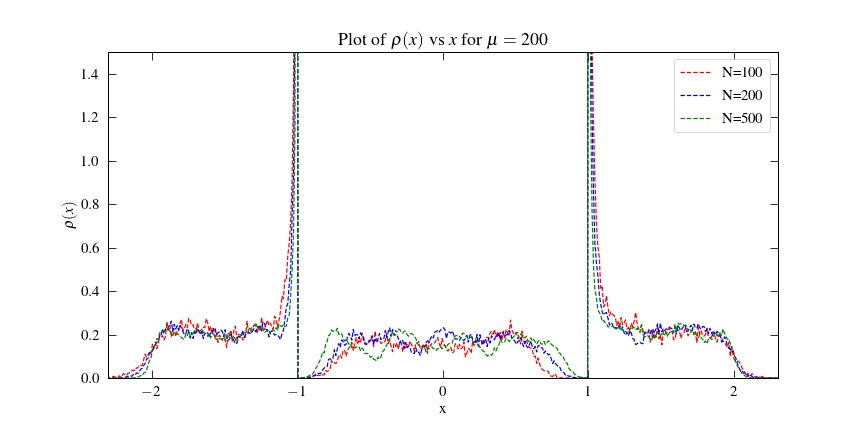
\includegraphics[width=0.8\columnwidth]{m200.jpg}
	\caption{Saddle point density profile for $\mu=200$}
	\label{fig:mu200}
\end{figure}
\begin{figure}[H]
	\centering
	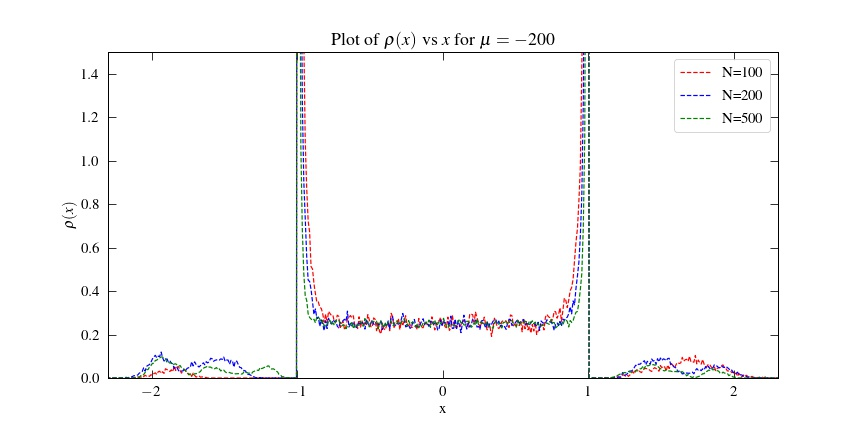
\includegraphics[width=0.8\columnwidth]{m-200.jpg}
	\caption{Saddle point density profile for $\mu=-200$}
	\label{fig:mu-200}
\end{figure}
Figures \ref{fig:mu0}-\ref{fig:mu-200} show the numerical results obtained for various values of $\mu$. 


\section{Calculating $\mathcal{P}(N_\mathcal{I})$}
From Appendix \ref{Analytical calculation}, we get two solutions for the saddle-point density. For the first set\eqref{set1}:
\begin{equation}
\rho^*(x) = \left\{ \,
\begin{IEEEeqnarraybox}[][c]{l?s}
\IEEEstrut
\frac{1}{4\alpha} & if $x\in [-2\alpha,-a)$, \\
\frac{\kappa_\mathcal{I}}{2a}+\frac{a-2\kappa_\mathcal{I}\alpha}{4\alpha}\{\delta(x+a)+\delta(x-a)\} & if $x \in [-a,a]$, \\
\frac{1}{4\alpha} & if $x\in ( a, 2\alpha]$.
\IEEEstrut
\end{IEEEeqnarraybox}
\right.
\end{equation}
The saddle-point action (eq.\eqref{eq-saddle_action}) then becomes
\begin{equation}
S(\alpha,\kappa_\mathcal{I},a) = \frac{1}{12\alpha}(a^3-4a^2\kappa_\mathcal{I}\alpha+4a\kappa_\mathcal{I}^2\alpha^2-8\alpha^3)
\end{equation}
The normalization factor
\begin{equation}
Z_N\approx \exp\left[-\beta N^2S(\alpha,\kappa_\mathcal{I}=0,a=0)\right] =\exp\left(\frac{2}{3}\beta N^2\alpha^2\right)
\end{equation}
Thus, in the limit of large $N$, the probability density of $N_\mathcal{I}$ is given by
$$
\mathcal{P}(N_\mathcal{I} = \kappa_\mathcal{I}N)= \frac{1}{Z_N}\exp\left[-\beta N^2S(\alpha,\kappa_\mathcal{I},a)\right]
$$
\begin{equation}
\boxed{\mathcal{P}(N_\mathcal{I} =\kappa_\mathcal{I}N)=\exp\left[-\beta N^2a\left(\frac{a^2}{12\alpha}+\frac{1}{3}\kappa_\mathcal{I}^2\alpha-\frac{1}{3}a\kappa_\mathcal{I}\right)\right]}\label{eq-final_pdf}
\end{equation}
for $-2\alpha\leq a\leq 2\alpha$. We can then check that for $a\geq 2\alpha$ and $\kappa = 1$,
\begin{equation}
\mathcal{P}(N_\mathcal{I} =N)= 1
\end{equation}
Thus, validating our calculation.
For the second set\eqref{set2}:

\begin{equation}
\rho^*(x) = \left\{ \,
\begin{IEEEeqnarraybox}[][c]{l?s}
\IEEEstrut
\frac{\kappa_\mathcal{I}}{2 a}+\frac{1-\kappa_\mathcal{I}}{2}\{\delta(x+a)+\delta(x-a)\} & if $x \in [-a,a]$, \\
0 & $\textrm{otherwise}$.
\IEEEstrut
\end{IEEEeqnarraybox}
\right.
\end{equation}
The saddle-point action (eq.\eqref{eq-saddle_action}) becomes
\begin{equation}
S(\alpha,\kappa_\mathcal{I},a) = \frac{a}{6}\left[a(3-2\kappa_\mathcal{I})-2\alpha(3-\kappa_\mathcal{I}^2)\right]
\end{equation}
which is normalized. In the limit of large $N$, the probability density of $N_\mathcal{I}$ is given by
\begin{equation}
\boxed{\mathcal{P}(N_\mathcal{I} =\kappa_\mathcal{I}N)=\exp\left[-\frac{\beta N^2a}{6}\left(a(3-2\kappa_\mathcal{I})-2\alpha(3-\kappa_\mathcal{I}^2)\right)\right]}\label{eq-final_pdf2}
\end{equation}

\section{Conclusion}
We have calculated the probability distribution of $N_\mathcal{I}$ particles within a symmetric interval $\mathcal{I}$. The analytical calculations for the first set agree asymptotically with results of Dhar et.al\cite{ref:dhar}. We verify eq.\eqref{eq-final_pdf} numerically by computing the distribution of $\kappa_\mathcal{I}$ for different values of $a$ and $N$. Results are shown in figs.\ref{fig:aa1}-\ref{fig:aa5}. Numerically eq.\eqref{eq-final_pdf2} could not be verified because of computational constriants (data going out of bounds). A further study on the second set of solution needs to be done.
\begin{figure}[H]
	\centering
	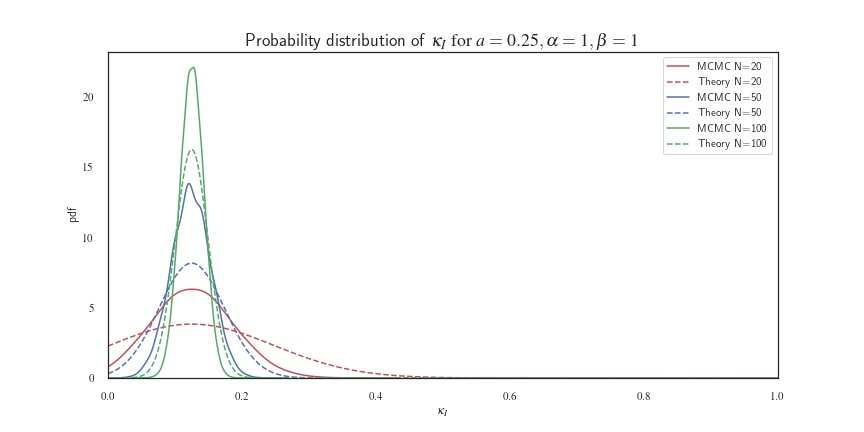
\includegraphics[width=0.8\columnwidth]{aa1.jpg}
	\caption{Distribution of $\kappa_\mathcal{I}$ for $a=0.25$}
	\label{fig:aa1}
\end{figure}
\begin{figure}[H]
	\centering
	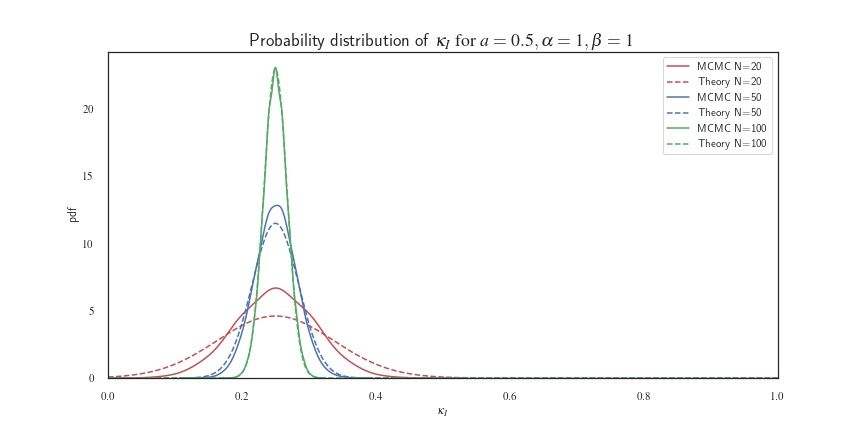
\includegraphics[width=0.8\columnwidth]{aa2.jpg}
	\caption{Distribution of $\kappa_\mathcal{I}$ for $a=0.5$}
	\label{fig:aa2}
\end{figure}
\begin{figure}[H]
	\centering
	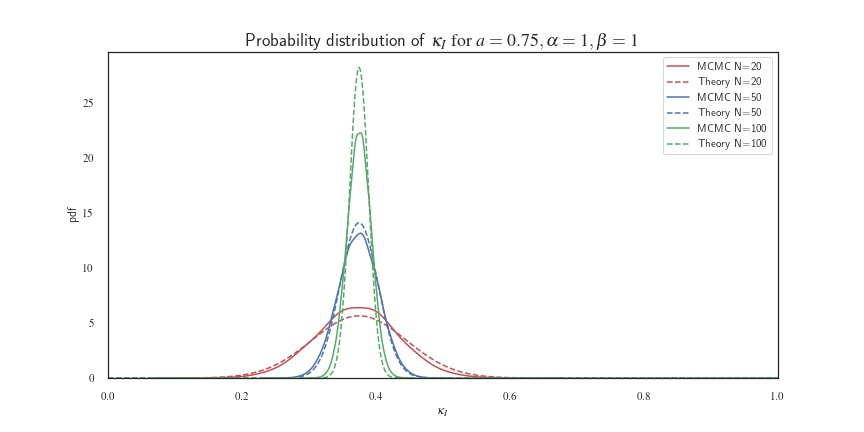
\includegraphics[width=0.8\columnwidth]{aa3.jpg}
	\caption{Distribution of $\kappa_\mathcal{I}$ for $a=0.75$}
	\label{fig:aa3}
\end{figure}
\begin{figure}[H]
	\centering
	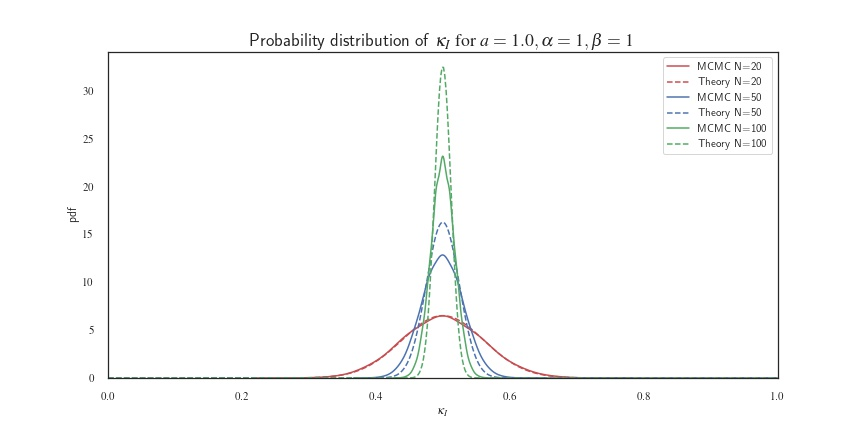
\includegraphics[width=0.8\columnwidth]{aa4.jpg}
	\caption{Distribution of $\kappa_\mathcal{I}$ for $a=1.0$}
	\label{fig:aa4}
\end{figure}
\begin{figure}[H]
	\centering
	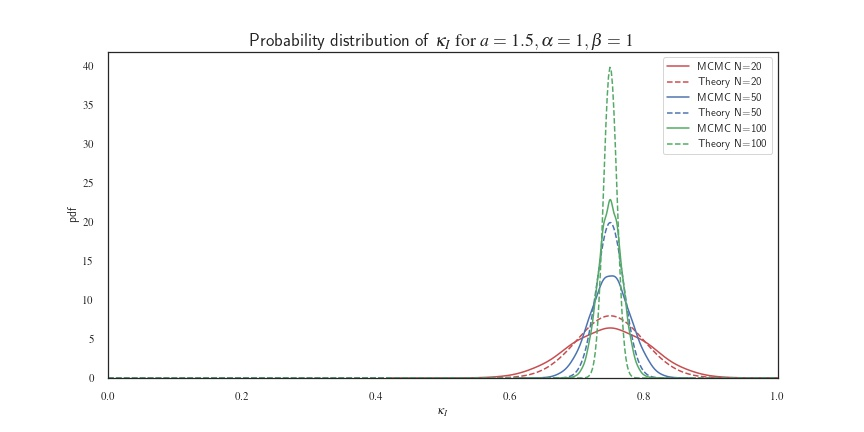
\includegraphics[width=0.8\columnwidth]{aa5.jpg}
	\caption{Distribution of $\kappa_\mathcal{I}$ for $a=1.5$}
	\label{fig:aa5}
\end{figure}


\appendix
\section{MCMC convergence}\label{MCMC convergence}
\begin{figure}[H]
\begin{subfigure}{.5\textwidth}
	\centering
	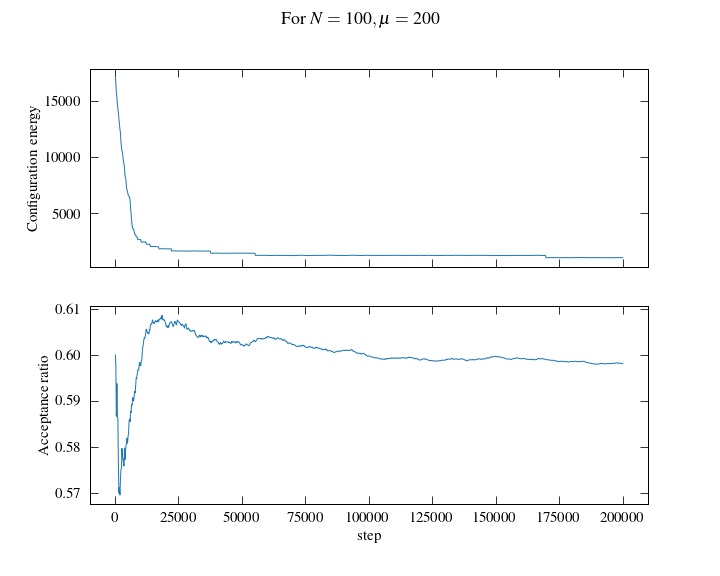
\includegraphics[scale=0.35]{convergence2.jpg}
	\caption{}
\end{subfigure}
\begin{subfigure}{.5\textwidth}
	\centering
	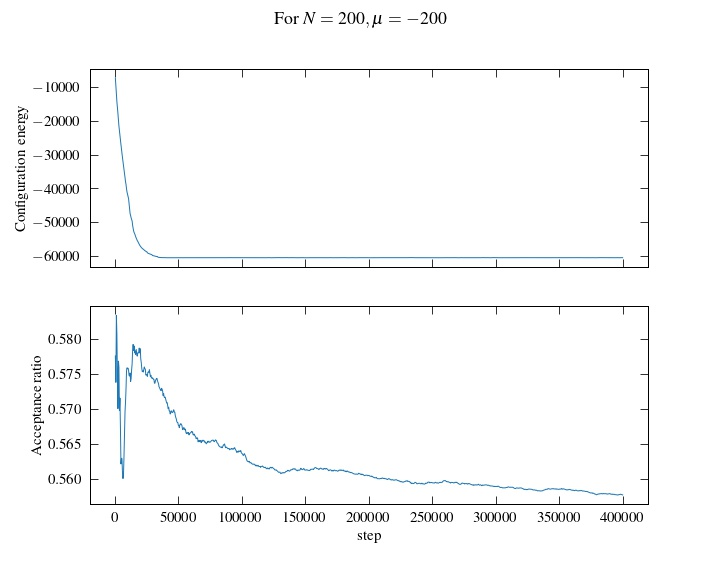
\includegraphics[scale=0.35]{convergence3.jpg}
	\caption{}
	%\label{fig:e_a}
\end{subfigure}
\newline
\begin{subfigure}{1.\textwidth}
	\centering
	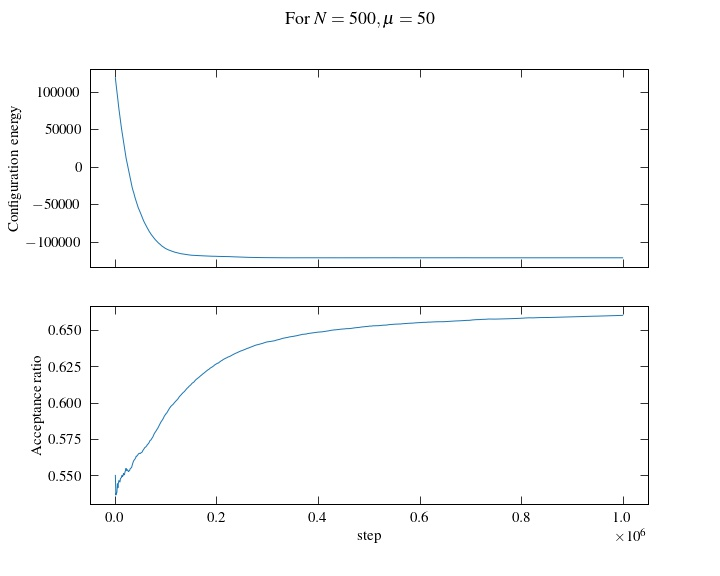
\includegraphics[width=0.8\columnwidth]{convergence1.jpg}
	\caption{}
\end{subfigure}
\caption{Plots indicating converegence of the MCMC algorithm for different values of $N$. The top panels show the energy at each realization (i.e. MCMC step). The bottom panels show the acceptance ratio at each realization. As expected, the acceptance ratio asymptotically becomes constant and energy reaches a minimum.}
\end{figure}


\section{Analytical calculation of the saddle point density}\label{Analytical calculation}
We are required to extremize the following action
\begin{align}
S[\rho,\mu,\eta]=&\int_{-\infty}^\infty\rho (x)\frac{x^2}{2}\,dx-\alpha\int_{-\infty}^\infty\,dx\int_{-\infty}^\infty \, dx'\rho (x)\rho (x')|x-x'|\nonumber\\
&+\mu\left[\int_{-a}^{a}\rho(x)\,dx-\kappa_I\right]+\eta\left[\int_{-\infty}^\infty\rho (x) \, dx-1\right]
\end{align}

Motivated by the numerical results, we consider the following ansatz for the saddle point density, $\rho^*$
\begin{equation}
\rho^*(x) = \left\{ \,
\begin{IEEEeqnarraybox}[][c]{l?s}
\IEEEstrut
A & if $x\in [-L,-a)$, \\
B+\lambda\{\delta(x+a)+\delta(x-a)\} & if $x \in [-a,a]$, \\
A & if $x\in ( a, L]$.
\IEEEstrut
\end{IEEEeqnarraybox}
\right.
\end{equation}
where $A$ and $B$ are constants and $\lambda$ represents the strength of the dirac-delta function at the walls of the interval. Thus, we have the following unknown parameters to determine: $A,B,\lambda,\mu, \eta \textrm{ and }L$. We insert the saddle point density ansatz into the action. A term-by-term calculation is done as given below.

The first term becomes,
\begin{align}
\int_{-\infty}^\infty\rho^*(x)\frac{x^2}{2}\,dx & = \frac{A}{2}\int_{-L}^{-a}x^2\,dx+\frac{B}{2}\int_{-a}^ax^2\,dx+\frac{A}{2}\int_{a}^{L}x^2\,dx+\lambda a^2\nonumber\\
& = \frac{A}{3}(L^3-a^3)+\frac{B}{3}a^3 +\lambda a^2 \label{e1}
\end{align}

The second term
\begin{align}
&-\alpha\int_{-\infty}^\infty\,dx\int_{-\infty}^\infty\,dx'\rho^*(x)\rho^*(x')|x-x'|=\nonumber\\
&-\alpha\int_{-L}^{-a}A\,dx\left[A\int_{-L}^{-a}|x-x'|\,dx'+B\int_{-a}^a|x-x'|\,dx'+A\int_{a}^{L}|x-x'|\,dx'+\lambda\left(|x-a|+|x+a|\right)\right]\nonumber\\
&-\alpha\int_{-a}^{a}B\,dx\left[A\int_{-L}^{-a}|x-x'|\,dx'+B\int_{-a}^a|x-x'|\,dx'+A\int_{a}^{L}|x-x'|\,dx'+\lambda\left(|x-a|+|x+a|\right)\right]\nonumber\\
&-\alpha\int_{a}^{L}A\,dx\left[A\int_{-L}^{-a}|x-x'|\,dx'+B\int_{-a}^a|x-x'|\,dx'+A\int_{a}^{L}|x-x'|\,dx'+\lambda\left(|x-a|+|x+a|\right)\right]\nonumber\\
&-\alpha\lambda[A\int_{-L}^{-a}\left(|x-a|+|x+a|\right)\,dx+B\int_{-a}^a\left(|x-a|+|x+a|\right)\,dx+A\int_{a}^{L}\left(|x-a|+|x+a|\right)\,dx'\nonumber\\
&+\lambda\int(\delta(x+a)+\delta(x-a))\left(|x-a|+|x+a|\right)\,dx]\nonumber\\
&\implies -\alpha\int_{-\infty}^\infty\,dx\int_{-\infty}^\infty\,dx'\rho^*(x)\rho^*(x')|x-x'|=\nonumber\\
&-2\alpha A\left[\frac{A}{3}(L-a)^3+A(L^2-a^2)(L-a)+Ba(L^2-a^2)+\lambda(L^2-a^2)\right]\nonumber\\
&-\alpha B\left[2Aa(L^2-a^2)+\frac{8}{3}Ba^3+4\lambda a^2\right]\nonumber\\
&-\alpha\lambda\left[2A(L^2-a^2)+4Ba^2+4a\lambda\right]\label{e2}
\end{align}

The third term
\begin{equation}
\mu\left[\int_{-a}^a\rho^*(x)\,dx-\kappa_\mathcal{I}\right]=\mu\left(2Ba-\kappa_\mathcal{I}\right)\label{e3}
\end{equation}

The fourth term
\begin{equation}
\eta\left[\int_{-L}^{L}\rho^*(x)dx-1\right]=\eta\left[2A(L-a)+2Ba+2\lambda-1\right]\label{e4}
\end{equation}

Adding equations \eqref{e1},\eqref{e2},\eqref{e3} and \eqref{e4}, we get
\begin{align}
S[\rho^*,\mu,\eta] = & \frac{A}{3}(L^3-a^3)+\frac{B}{3}a^3+\lambda a^2-\frac{2}{3}\alpha A^2(L-a)^3-2\alpha A^2(L-a)(L^2-a^2)\nonumber\\
&-4\alpha ABa(L^2-a^2)-\frac{8}{3}\alpha B^2a^3-4\alpha\lambda A(L^2-a^2)-8\alpha\lambda B a^2\nonumber\\
&-4\alpha\lambda^2a+\mu(2Ba-\kappa_\mathcal{I})+\eta\left[2A(L-a)+2Ba+2\lambda-1\right]\label{eq-saddle_action}
\end{align}
We now minimise $S[\rho^*,\mu,\eta]$ w.r.t. $A,B,\lambda,\mu,\eta \textrm{ and } L$ to get
\begin{align}
&\frac{\partial S}{\partial A}=0\nonumber\\
\implies &\frac{L-a}{3}[L^2(1-16\alpha A)+a^2(1+8\alpha A-12 \alpha B)+6\eta-12\alpha\lambda L\nonumber\\&+a(L+8\alpha A L-12\alpha BL-12\alpha \lambda)]=0\label{min1}\\
&\frac{\partial S}{\partial B} =0\nonumber\\
\implies & \frac{a}{3}\left[a^2(1+12\alpha A-16\alpha B)-24\alpha\lambda a-6(2\alpha AL^2-\eta-\mu)\right]=0\label{min2}\\
&\frac{\partial S}{\partial \lambda} =0\nonumber\\
\implies &-4\alpha AL^2+a^2(1+4\alpha A-8\alpha B)+2\eta-8\alpha\lambda a=0\label{min3}\\
&\frac{\partial S}{\partial \mu} =0\nonumber\\
\implies & 2aB-\kappa_\mathcal{I}=0\label{min4}\\
&\frac{\partial S}{\partial \eta} =0\nonumber\\
\implies & 2A(L-a)+2Ba+2\lambda-1 =0\label{min5}\\
&\frac{\partial S}{\partial L} =0\nonumber\\
\implies & A[L^2(1-8\alpha A)+2\eta +8\alpha L\{a(A-B)-\lambda\}]=0\label{min6}
\end{align}
Solving equations \eqref{min1}-\eqref{min6} simultaneously gives two sets of solutions. The first set is
\begin{subequations}
\begin{empheq}[box=\widefbox]{align}
  A & = \frac{1}{4\alpha} \\
  B & = \frac{\kappa_\mathcal{I}}{2a}\\
  \lambda & = \frac{a-2\kappa_\mathcal{I}\alpha}{4\alpha}\\
  \eta & = 2\alpha^2\\
  \mu & = \frac{1}{3}a(a-2\kappa_\mathcal{I}\alpha)\\
  L & = 2\alpha
\end{empheq}\label{set1}
\end{subequations}
and the second set is
\begin{subequations}
\begin{empheq}[box=\widefbox]{align}
  A & = 0 \\
  B & = \frac{\kappa_\mathcal{I}}{2a}\\
  \lambda & = \frac{1-\kappa_\mathcal{I}}{2}\\
  \eta & = -\frac{1}{2}a(a-4\alpha)\\
  \mu & = \frac{1}{3}a(a-2\kappa_\mathcal{I}\alpha)\\
  L & = a
\end{empheq}\label{set2}
\end{subequations}


\section*{Acknowledgements}
Uddeepta would like to convey his gratitude towards Prof. Kundu for his mentorship.

\begin{thebibliography} {9}
\bibitem{ref:marino} Marino, R., et.al., \href{https://journals.aps.org/pre/abstract/10.1103/PhysRevE.94.032115}{Phys. Rev. E 94,032115 (2016).}
\bibitem{ref:dhar} Dhar, A., et.al., \href{https://iopscience.iop.org/article/10.1088/1751-8121/aac75f/meta}{J. Phys. A: Math. Theor. 51 295001 (2018).}
\bibitem{ref:forrester} Forrester, P.J., \textit{Log-Gases and Random Matrices}, London Mathematical Society, London (2010).
\bibitem{ref:oxford} Akemann, G., Baik, J.,\& Di Francesco, P.,\textit{The Oxford Handbook of Random Matrix Theory}, OUP, Oxford (2015).
\bibitem{ref:mehta} Mehta, M.L.,\textit{Random Matrices}, Elsevier (2004).

\end{thebibliography}

\end{document}